\documentclass[aspectratio=169,11pt]{beamer}

\def\courseTitle{Industrial Security (Bachelor)}
\def\courseSubtitle{Section 08 -- Defense in Depth}
\def\sectionNumber{08}
\def\sectionTitle{Defense in Depth}

% =====================================================================
% Industrial Security lecture series -- modern Beamer preamble.
%
% Each slide deck must define the following BEFORE \input{}-ing this:
%   \def\courseTitle{...}        e.g. Industrial Security (Bachelor)
%   \def\courseSubtitle{...}     e.g. Section 3 -- Network Architecture
%   \def\sectionNumber{...}      e.g. 03
%   \def\sectionTitle{...}       e.g. Industrial Network Architectures
%
% Optional:
%   \def\courseAuthor{...}       defaults to "Lecture Notes"
%   \def\courseInstitute{...}    defaults to "Department of Computer Science"
%   \def\companyLogo{...}        path to a logo image (PDF/PNG/JPG).
%
% Callout macros (use anywhere inside a frame):
%   \begin{notebox}{title}      ... \end{notebox}
%   \begin{importantbox}{title} ... \end{importantbox}
%   \begin{warningbox}{title}   ... \end{warningbox}
%   \begin{tipbox}{title}       ... \end{tipbox}
%   \begin{defbox}{title}       ... \end{defbox}
%   \begin{takeawaybox}{title}  ... \end{takeawaybox}
%   \begin{quotebox}            ... \end{quotebox}
% =====================================================================

% --- Speaker-notes mode (toggled by Makefile via -usepretex) ----------
% When notesmode=1, build a side-by-side slide+notes PDF for the
% lecturer. When unset/0, build the clean slides-only PDF.
\providecommand{\notesmode}{0}
\ifnum\notesmode=1
  \usepackage{pgfpages}
  \setbeameroption{show notes on second screen=right}
  \setbeamerfont{note page}{size=\small}
\fi

\usepackage[utf8]{inputenc}
\usepackage[T1]{fontenc}
\usepackage[english]{babel}
% Modern type pair: IBM Plex Sans for text, IBM Plex Mono for code.
% Math stays in lmodern; Plex is the dominant family on every text frame.
\usepackage{plex-sans}
\usepackage{plex-mono}
\renewcommand{\familydefault}{\sfdefault}
\usepackage[activate={true,nocompatibility},final,tracking=true,kerning=true,spacing=true,factor=1100,stretch=10,shrink=10]{microtype}
\usepackage{graphicx}
\usepackage{listings}
\usepackage{xcolor}
\usepackage{colortbl}
\usepackage{tikz}
\usepackage{booktabs}
\usepackage{array}
\usepackage{hyperref}
\usepackage{amsmath}
\usepackage{amssymb}
\usepackage{tcolorbox}
\tcbuselibrary{skins, breakable, raster}
\usepackage{fontawesome5}

% =====================================================================
% Shared TikZ styles for the Industrial Security lecture series.
% Loaded by every slide deck and exercise sheet that uses TikZ.
% =====================================================================

\usetikzlibrary{
  arrows.meta,
  shapes,
  shapes.geometric,
  shapes.symbols,
  shapes.multipart,
  positioning,
  fit,
  calc,
  backgrounds,
  decorations.pathmorphing,
  decorations.pathreplacing,
  decorations.text,
  patterns,
  matrix,
  shadows
}

% --- colour palette --------------------------------------------------
\definecolor{isOT}{HTML}{1F4E79}     % OT (deep blue)
\definecolor{isIT}{HTML}{6F2DA8}     % IT (purple)
\definecolor{isSafety}{HTML}{C00000} % safety red
\definecolor{isNet}{HTML}{2E7D32}    % network green
\definecolor{isAttack}{HTML}{B23A48} % attack red
\definecolor{isAccent}{HTML}{E08E0B} % amber
\definecolor{isMute}{HTML}{6B6B6B}   % grey
\definecolor{isLight}{HTML}{EDF2F8}  % light background
\definecolor{isPLC}{HTML}{2C5282}
\definecolor{isHMI}{HTML}{2F855A}
\definecolor{isSCADA}{HTML}{6B46C1}

% --- generic node styles --------------------------------------------
\tikzset{
  isnode/.style={
    draw, rounded corners=2pt, minimum height=8mm, minimum width=18mm,
    font=\small, align=center, thick
  },
  isbox/.style={isnode, fill=isLight},
  plc/.style={isnode, fill=isPLC!15, draw=isPLC, thick},
  hmi/.style={isnode, fill=isHMI!15, draw=isHMI, thick},
  scada/.style={isnode, fill=isSCADA!15, draw=isSCADA, thick},
  sensor/.style={isnode, fill=isNet!10, draw=isNet, minimum height=6mm, minimum width=14mm, font=\scriptsize},
  actuator/.style={isnode, fill=isAccent!15, draw=isAccent, minimum height=6mm, minimum width=14mm, font=\scriptsize},
  firewall/.style={isnode, fill=isAttack!15, draw=isAttack, thick},
  server/.style={isnode, fill=isMute!15, draw=isMute!80, thick},
  switch/.style={isnode, fill=isLight, draw=black!60, minimum height=6mm, minimum width=14mm, font=\scriptsize},
  workstation/.style={isnode, fill=white, draw=isOT, thick},
  attacker/.style={isnode, fill=isAttack!20, draw=isAttack, thick, font=\small\bfseries},
  inetnode/.style={draw, ellipse, minimum width=24mm, minimum height=10mm, font=\scriptsize, fill=isLight, thick},
  process/.style={isnode, fill=isOT!15, draw=isOT, thick, minimum width=24mm},
  zone/.style={
    draw, rounded corners=4pt, thick, dashed, inner sep=4mm
  },
  conduit/.style={-{Stealth[length=2.5mm]}, thick, isNet!80!black},
  attack/.style={-{Stealth[length=2.5mm]}, thick, isAttack, dashed},
  flow/.style={-{Stealth[length=2.5mm]}, thick, isOT!70!black},
  netline/.style={thick, black!60},
  axisline/.style={-{Stealth[length=2mm]}, thick, black!70},
  tag/.style={font=\scriptsize\itshape, fill=white, inner sep=1pt},
  level/.style={
    draw, fill=isLight, minimum width=0.85\linewidth, minimum height=8mm,
    font=\small, anchor=west
  },
  brace/.style={decorate, decoration={brace, amplitude=4pt, raise=2pt}},
  legendbox/.style={draw, rounded corners=2pt, fill=isLight, inner sep=2mm, font=\scriptsize, align=left}
}

% --- handy macros ----------------------------------------------------
% \plcicon, \hmiicon etc as simple labelled boxes; useful inline.
\newcommand{\plcicon}[1][PLC]{\tikz[baseline=-0.6ex]{\node[plc, minimum width=10mm, minimum height=5mm, font=\scriptsize, inner sep=1pt]{#1};}}
\newcommand{\hmiicon}[1][HMI]{\tikz[baseline=-0.6ex]{\node[hmi, minimum width=10mm, minimum height=5mm, font=\scriptsize, inner sep=1pt]{#1};}}
\newcommand{\fwicon}[1][FW]{\tikz[baseline=-0.6ex]{\node[firewall, minimum width=10mm, minimum height=5mm, font=\scriptsize, inner sep=1pt]{#1};}}


\graphicspath{{.}{../../../template/}}

% --- defaults --------------------------------------------------------
\providecommand{\courseAuthor}{Lecture Notes}
\providecommand{\courseInstitute}{Department of Computer Science}
\providecommand{\companyLogo}{logo}

% --- modern palette --------------------------------------------------
\definecolor{slideAccent}{HTML}{1F4E79}       % primary navy
\definecolor{slideSecondary}{HTML}{E08E0B}    % amber accent

% --- Corporate branding overrides ------------------------------------
% A user-editable `branding.tex` at the repo root can override the
% logo path, author/institute lines, and brand colours. If the file is
% missing the built-in defaults above stay in effect.
\IfFileExists{../../../branding.tex}{% =====================================================================
% Corporate / institutional branding -- single file to customise the
% look of the entire course (slides, notes, exercises, labs).
%
% HOW TO REBRAND IN UNDER A MINUTE:
%   1. Replace `branding/logo.pdf` with your own logo
%      (PDF preferred; PNG and JPG also work -- name it `logo.<ext>`).
%   2. (Optional) change the two colours below to your brand palette.
%   3. (Optional) override the author/institute lines below.
%   4. Re-run `make` at the repo root. That's it.
%
% Everything in this file has sensible defaults; you can delete a line
% to fall back to the built-in defaults, or comment it out.
%
% This file is loaded automatically by the slides, exercise, and lab
% preambles -- you never need to \input it manually.
% =====================================================================

% --- Logo --------------------------------------------------------------
% Path is resolved from each leaf-build directory; the default points at
% the shared `branding/` folder at the repo root. If you put your logo
% somewhere else, set the full or relative path here (without extension):
\renewcommand{\companyLogo}{../../../branding/logo}

% --- Author / institute (appears on the title page footer) ------------
\renewcommand{\courseAuthor}{}
\renewcommand{\courseInstitute}{}

% --- Brand colours ----------------------------------------------------
% slideAccent      = primary brand colour (title bands, accent rule)
% slideSecondary   = secondary brand colour (section badge, highlight)
% Both use HTML hex codes. Keep enough contrast against white text.
\definecolor{slideAccent}{HTML}{00205B}      % deep navy
\definecolor{slideSecondary}{HTML}{00A0DC}   % light blue accent
}{}
\definecolor{slideTitle}{HTML}{0F2A44}        % near-black navy
\definecolor{slideMuted}{HTML}{6B6B6B}
\definecolor{slideBg}{HTML}{FFFFFF}
\definecolor{slidePanel}{HTML}{F4F7FB}
\definecolor{slideRule}{HTML}{D6DEE8}

% Callout colours
\definecolor{calNote}{HTML}{1F4E79}
\definecolor{calImportant}{HTML}{B23A48}
\definecolor{calWarning}{HTML}{C77700}
\definecolor{calTip}{HTML}{2E7D32}
\definecolor{calDef}{HTML}{6B46C1}
\definecolor{calTake}{HTML}{0F2A44}

% --- beamer theme ---------------------------------------------------
\useinnertheme{rectangles}
\usefonttheme{professionalfonts}

\setbeamertemplate{navigation symbols}{}
\setbeamertemplate{itemize items}[circle]
\setbeamertemplate{enumerate items}[default]
\setbeamertemplate{section in toc}[ball numbered]
\setbeamercolor{section in toc}{fg=slideTitle}

% Colours
\setbeamercolor{normal text}{fg=slideTitle, bg=slideBg}
\setbeamercolor{title}{fg=slideAccent}
\setbeamercolor{subtitle}{fg=slideMuted}
\setbeamercolor{frametitle}{fg=slideAccent}
\setbeamercolor{structure}{fg=slideAccent}
\setbeamercolor{itemize item}{fg=slideAccent}
\setbeamercolor{itemize subitem}{fg=slideSecondary}
\setbeamercolor{block title}{fg=white, bg=slideAccent}
\setbeamercolor{block body}{fg=slideTitle, bg=slidePanel}
\setbeamercolor{alerted text}{fg=slideSecondary}

% Fonts
\setbeamerfont{title}{series=\bfseries, size=\Large}
\setbeamerfont{subtitle}{series=\mdseries, size=\normalsize}
\setbeamerfont{frametitle}{series=\bfseries, size=\large}
\setbeamerfont{block title}{series=\bfseries, size=\normalsize}
\setbeamerfont{footline}{size=\tiny}

% --- frametitle: title bar + accent underline + section badge -------
% The accent rules are wrapped in a zero-width box so they never
% contribute to the surrounding hbox width (no Overfull warnings).
\setbeamertemplate{frametitle}{%
  \nointerlineskip
  \begin{beamercolorbox}[wd=\paperwidth, ht=2.8ex, dp=1.6ex, leftskip=1.2em, rightskip=1.2em]{frametitle}%
    \usebeamerfont{frametitle}\insertframetitle%
    \hfill
    {\color{slideMuted}\small \sectionNumber}%
  \end{beamercolorbox}%
  \nointerlineskip
  \makebox[0pt][l]{\hspace*{1.2em}\textcolor{slideSecondary}{\rule{2.5em}{1pt}}\textcolor{slideAccent}{\rule{\dimexpr\paperwidth-3.7em\relax}{1pt}}}%
  \par\vskip4pt
}

% --- footer ---------------------------------------------------------
\defbeamertemplate*{footline}{is-footer}{%
  \leavevmode%
  \hbox{%
    \begin{beamercolorbox}[wd=.55\paperwidth, ht=2.4ex, dp=1ex, leftskip=1em]{author in head/foot}%
      {\color{slideMuted}\tiny \courseTitle{} \;\; $\bullet$ \;\; Section \sectionNumber{} -- \sectionTitle}%
    \end{beamercolorbox}%
    \begin{beamercolorbox}[wd=.45\paperwidth, ht=2.4ex, dp=1ex, rightskip=1em]{title in head/foot}%
      \hfill {\color{slideMuted}\tiny \insertframenumber{} / \inserttotalframenumber}%
    \end{beamercolorbox}%
  }%
  \vskip2pt
}

% --- listings -------------------------------------------------------
\definecolor{codebg}{HTML}{F4F7FB}
\definecolor{codekw}{HTML}{0F2A44}
\definecolor{codestr}{HTML}{8B3A3A}
\definecolor{codecom}{HTML}{5A7D54}

\lstset{
    backgroundcolor=\color{codebg},
    basicstyle=\ttfamily\scriptsize\color{slideTitle},
    keywordstyle=\color{codekw}\bfseries,
    stringstyle=\color{codestr},
    commentstyle=\color{codecom}\itshape,
    breaklines=true,
    frame=leftline,
    framerule=2pt,
    rulecolor=\color{slideAccent},
    numbers=left,
    numberstyle=\tiny\color{slideMuted},
    numbersep=8pt,
    showstringspaces=false,
    tabsize=2,
    captionpos=b,
    xleftmargin=0.6em
}

% --- callout boxes --------------------------------------------------
% Shared base style for all callout boxes.
% Subtle drop shadow gives the boxes a hint of elevation without distraction.
\tcbset{
  isCallout/.style={
    enhanced, breakable, sharp corners=northeast,
    arc=2pt, boxrule=0pt,
    leftrule=3pt,
    fonttitle=\bfseries\small,
    coltitle=white,
    fontupper=\small,
    left=2mm, right=2mm, top=1.5mm, bottom=1.5mm,
    drop fuzzy shadow=black!30,
    title={#1}
  }
}

\newtcolorbox{notebox}[1]{
  isCallout={#1},
  colback=calNote!8, colframe=calNote, leftrule=3pt,
  colbacktitle=calNote, attach boxed title to top left={xshift=2mm, yshift=-1.2mm},
  boxed title style={colback=calNote, arc=1pt, boxrule=0pt, left=2mm, right=2mm, top=0.5mm, bottom=0.5mm}
}

\newtcolorbox{importantbox}[1]{
  isCallout={#1},
  colback=calImportant!7, colframe=calImportant, leftrule=4pt,
  colbacktitle=calImportant, attach boxed title to top left={xshift=2mm, yshift=-1.2mm},
  boxed title style={colback=calImportant, arc=1pt, boxrule=0pt, left=2mm, right=2mm, top=0.5mm, bottom=0.5mm}
}

\newtcolorbox{warningbox}[1]{
  isCallout={#1},
  colback=calWarning!10, colframe=calWarning, leftrule=4pt,
  colbacktitle=calWarning, attach boxed title to top left={xshift=2mm, yshift=-1.2mm},
  boxed title style={colback=calWarning, arc=1pt, boxrule=0pt, left=2mm, right=2mm, top=0.5mm, bottom=0.5mm}
}

% Alias warnbox = warningbox, with an optional title (default = "Caution")
\newtcolorbox{warnbox}[1][Caution]{
  isCallout={#1},
  colback=calWarning!10, colframe=calWarning, leftrule=4pt,
  colbacktitle=calWarning, attach boxed title to top left={xshift=2mm, yshift=-1.2mm},
  boxed title style={colback=calWarning, arc=1pt, boxrule=0pt, left=2mm, right=2mm, top=0.5mm, bottom=0.5mm}
}

\newtcolorbox{tipbox}[1]{
  isCallout={#1},
  colback=calTip!8, colframe=calTip, leftrule=3pt,
  colbacktitle=calTip, attach boxed title to top left={xshift=2mm, yshift=-1.2mm},
  boxed title style={colback=calTip, arc=1pt, boxrule=0pt, left=2mm, right=2mm, top=0.5mm, bottom=0.5mm}
}

\newtcolorbox{defbox}[1]{
  isCallout={#1},
  colback=calDef!8, colframe=calDef, leftrule=3pt,
  colbacktitle=calDef, attach boxed title to top left={xshift=2mm, yshift=-1.2mm},
  boxed title style={colback=calDef, arc=1pt, boxrule=0pt, left=2mm, right=2mm, top=0.5mm, bottom=0.5mm}
}

\newtcolorbox{takeawaybox}[1]{
  enhanced, breakable, arc=3pt, boxrule=0pt,
  colback=calTake!7, colframe=calTake,
  toptitle=2mm, bottomtitle=2mm,
  fonttitle=\bfseries\normalsize, coltitle=white,
  colbacktitle=calTake,
  fontupper=\small,
  title={\faStar~Key Takeaway: #1},
  left=3mm, right=3mm, top=2mm, bottom=2mm
}

\newtcolorbox{quotebox}{
  enhanced, breakable, arc=2pt, boxrule=0pt,
  colback=slidePanel, colframe=slideMuted,
  leftrule=3pt, top=2mm, bottom=2mm, left=3mm, right=3mm,
  fontupper=\itshape\small,
}

% Convenience: inline highlight badge
\newcommand{\remembertag}{\tikz[baseline=-0.7ex]\node[fill=calImportant, text=white, font=\scriptsize\bfseries, rounded corners=2pt, inner sep=2pt]{REMEMBER};}
\newcommand{\tldr}{\tikz[baseline=-0.7ex]\node[fill=calTake, text=white, font=\scriptsize\bfseries, rounded corners=2pt, inner sep=2pt]{TL;DR};}

% Source attribution: tiny grey line, anchored bottom-left of the content area
% Usage:  \source{Symantec, \emph{W32.Stuxnet Dossier} v1.4, 2011.}
% Multiple sources:  \source{X.\ Y., 2018; Z, 2020.}
\newcommand{\source}[1]{%
  \par\nointerlineskip\vspace{0.4mm}%
  {\color{slideMuted}\fontsize{5.5}{6.5}\selectfont\textit{Source:} #1\par}%
}

% References slide: aggregate citations + further reading at the end of a section.
% Usage:  \referencesframe{ \item ... \item ... }
% The `frame` environment must be written literally in the deck, so this is a
% macro rather than a wrapper environment (beamer collects the frame body and
% trips over \newenvironment wrappers).
%
% allowframebreakstemplate=\insertcontinuationcount silences the trailing roman
% numeral when content fits on a single page.
\setbeamertemplate{frametitle continuation}[from second]
\newcommand{\referencesframe}[1]{%
  \begin{frame}[allowframebreaks]{References -- Section \sectionNumber}
    \fontsize{7.5}{9}\selectfont
    \setlength{\itemsep}{1pt}
    \begin{itemize}#1\end{itemize}
  \end{frame}%
}

% --- title page -----------------------------------------------------
\title[\courseTitle]{\courseTitle}
\subtitle{\courseSubtitle}
\author{\courseAuthor}
\institute{\courseInstitute}
\date{}

% Logo lookup: try the section directory, then the shared template/.
\newcommand{\showlogo}[1][2cm]{%
  \IfFileExists{\companyLogo.pdf}{\includegraphics[width=#1]{\companyLogo}}{%
    \IfFileExists{\companyLogo.png}{\includegraphics[width=#1]{\companyLogo}}{%
      \IfFileExists{\companyLogo.jpg}{\includegraphics[width=#1]{\companyLogo}}{%
        \IfFileExists{../../../template/\companyLogo.pdf}{\includegraphics[width=#1]{../../../template/\companyLogo}}{%
          \rule{0pt}{0pt}}}}}}

\setbeamertemplate{title page}{%
  \begin{tikzpicture}[remember picture, overlay]
    % accent band (taller to fit wrapped titles)
    \fill[slideAccent] (current page.north west) rectangle ([yshift=-3.4cm]current page.north east);
    \fill[slideSecondary] ([yshift=-3.4cm]current page.north west) rectangle ([yshift=-3.55cm]current page.north east);
    % section badge
    \node[fill=slideSecondary, text=white, font=\bfseries\normalsize, rounded corners=3pt, inner sep=4pt, anchor=north west]
      at ([xshift=1.2cm, yshift=-0.7cm]current page.north west) {Section \sectionNumber};
    % Course title (wraps if long)
    \node[anchor=north west, text=white, font=\bfseries\Large, align=left, text width=11cm]
      at ([xshift=1.2cm, yshift=-1.5cm]current page.north west) {\courseTitle};
    % Subtitle (wraps; smaller, separated)
    \node[anchor=north west, text=white, font=\mdseries\small, align=left, text width=11cm]
      at ([xshift=1.2cm, yshift=-2.7cm]current page.north west) {\courseSubtitle};
    \node[anchor=north east] at ([xshift=-1.2cm, yshift=-1.0cm]current page.north east)
      {\showlogo[2cm]};
    \node[anchor=south west, text=slideMuted, font=\small, align=left, text width=11cm]
      at ([xshift=1.2cm, yshift=1.0cm]current page.south west)
      {\textbf{\sectionTitle}\\[2pt]\textit{\courseAuthor}\\{\scriptsize\courseInstitute}};
  \end{tikzpicture}
}

% --- helper macros --------------------------------------------------
\newcommand{\learningobjectives}[1]{%
  \begin{frame}{Learning Objectives}
    \begin{tipbox}{\faGraduationCap~By the end of this section you will be able to}
      \begin{itemize}\setlength{\itemsep}{2pt}#1\end{itemize}
    \end{tipbox}
  \end{frame}}

\newcommand{\sectionoverviewframe}{%
  \begin{frame}[plain,noframenumbering]
    \titlepage
  \end{frame}
  \begin{frame}{Outline -- Section \sectionNumber}
    \tableofcontents
  \end{frame}}

\AtBeginSection[]{%
  \begin{frame}[plain,noframenumbering]
    \begin{tikzpicture}[remember picture, overlay]
      \fill[slideAccent] (current page.north west) rectangle (current page.south east);
      \fill[slideSecondary] ([yshift=-1pt]current page.center -| current page.west)
                            rectangle ([yshift=1pt]current page.center -| current page.east);
      \node[text=white, font=\scriptsize, anchor=south west]
        at ([xshift=1.2cm, yshift=1.0cm]current page.south west)
        {Section \sectionNumber{} -- \sectionTitle};
      \node[text=slideSecondary, font=\bfseries\Huge, anchor=south]
        at ([yshift=0.4cm]current page.center)
        {\thesection};
      \node[text=white, font=\bfseries\LARGE, align=center, anchor=north, text width=12cm]
        at ([yshift=-0.6cm]current page.center)
        {\insertsection};
    \end{tikzpicture}
  \end{frame}}

\newcommand{\closingframe}{%
  \begin{frame}[plain,noframenumbering]
    \begin{tikzpicture}[remember picture, overlay]
      \fill[slideAccent] (current page.north west) rectangle (current page.south east);
      \node[text=white, font=\bfseries\Huge, anchor=center, align=center, text width=14cm]
        at ([yshift=8mm]current page.center) {End of Section \sectionNumber};
      \fill[slideSecondary] ([xshift=-1.5cm, yshift=-4mm]current page.center)
                            rectangle ([xshift=1.5cm, yshift=-6mm]current page.center);
      \node[text=white, font=\large, anchor=north, align=center, text width=14cm]
        at ([yshift=-1.2cm]current page.center) {\sectionTitle};
      \node[text=slideSecondary, font=\normalsize, anchor=south] at ([yshift=1.2cm]current page.south) {Questions and discussion};
      \node[anchor=south east] at ([xshift=-1cm, yshift=1cm]current page.south east) {\showlogo[1.5cm]};
    \end{tikzpicture}
  \end{frame}}


\begin{document}

\sectionoverviewframe

\learningobjectives{
  \item Apply defense-in-depth across people, process, and technology.
  \item Design layered controls for an ICS environment.
  \item Specify secure remote access patterns for vendors.
  \item Position passive ICS IDS and explain alert triage.
}

\section{Layered Controls}

\begin{frame}{The Defense-in-Depth Onion}
\vspace{-2mm}
\begin{columns}[T]
\column{0.5\textwidth}
\centering
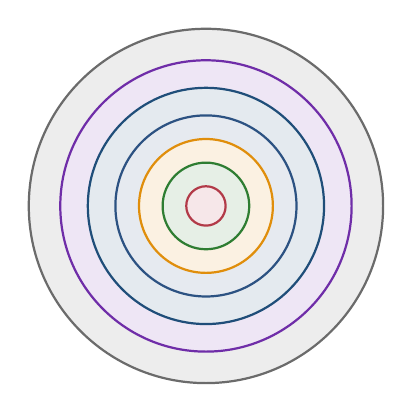
\begin{tikzpicture}[scale=0.5, transform shape]
  \foreach \R/\col in {
    4.5/isMute, 3.7/isIT, 3.0/isOT, 2.3/isPLC,
    1.7/isAccent, 1.1/isNet, 0.5/isAttack}{
    \draw[thick, fill=\col!12, draw=\col] (0,0) circle (\R);
  }
\end{tikzpicture}
\column{0.5\textwidth}
\vspace{1mm}
{\scriptsize\setlength{\itemsep}{1pt}
\begin{itemize}
  \item \textcolor{isMute}{$\blacksquare$} Policies \& procedures
  \item \textcolor{isIT}{$\blacksquare$} Physical security
  \item \textcolor{isOT}{$\blacksquare$} Network segmentation
  \item \textcolor{isPLC}{$\blacksquare$} Host hardening
  \item \textcolor{isAccent}{$\blacksquare$} Application \& RBAC
  \item \textcolor{isNet}{$\blacksquare$} Data \& backups
  \item \textcolor{isAttack}{$\blacksquare$} Monitoring \& IR
\end{itemize}}
\end{columns}
\vspace{1mm}
\begin{importantbox}{Layered}
A single failed layer should not equal a successful attack.
\end{importantbox}
\source{INL, \emph{Recommended Practice: Improving ICS Cybersecurity with Defense-in-Depth Strategies}, 2016 \textbar{} NIST SP 800-82 Rev.\,3, 2023.}
\note{
  Defense in depth is not ``more controls equals more safety.'' It is layered \emph{independence}: each layer must fail in a different way. Make this concrete: if your perimeter firewall, your internal firewall, and your endpoint AV all run the same Windows engine, you have one layer with three logos. The INL onion is useful as a checklist, not as a maturity ladder -- you do not earn the inner ring by completing the outer. Ask the room: what makes a layer truly \emph{independent}? The answer involves different vendors, different protocols, and different administrators.
}
\end{frame}

\begin{frame}{Hardening ICS Hosts}
\centering
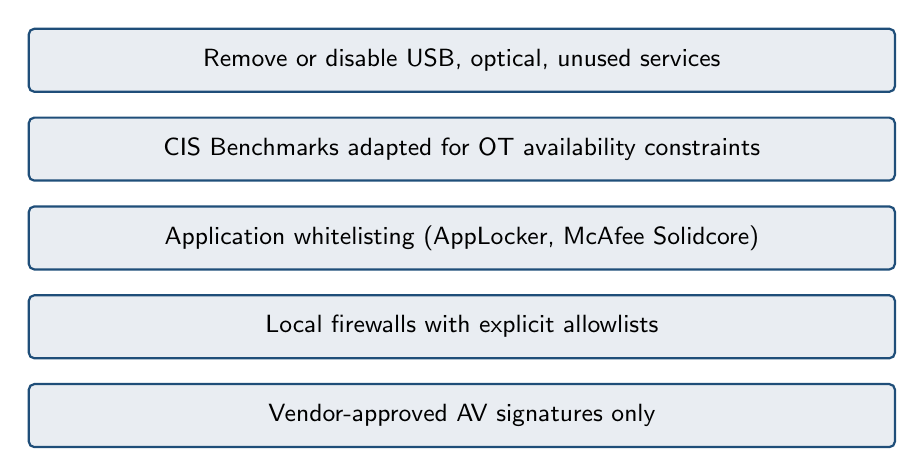
\begin{tikzpicture}[node distance=3mm]
  \node[isbox, fill=isOT!10, draw=isOT, minimum width=110mm, font=\small] (a) {Remove or disable USB, optical, unused services};
  \node[isbox, fill=isOT!10, draw=isOT, minimum width=110mm, font=\small, below=of a] (b) {CIS Benchmarks adapted for OT availability constraints};
  \node[isbox, fill=isOT!10, draw=isOT, minimum width=110mm, font=\small, below=of b] (c) {Application whitelisting (AppLocker, McAfee Solidcore)};
  \node[isbox, fill=isOT!10, draw=isOT, minimum width=110mm, font=\small, below=of c] (d) {Local firewalls with explicit allowlists};
  \node[isbox, fill=isOT!10, draw=isOT, minimum width=110mm, font=\small, below=of d] (e) {Vendor-approved AV signatures only};
\end{tikzpicture}
\note{
  Hardening on a static HMI is a near-perfect fit: the binary set never changes, so application allow-listing (AppLocker, McAfee Solidcore, Carbon Black App Control) actually holds. The catch is the CIS Benchmark line -- you cannot apply the IT profile blindly because half of it breaks OPC, breaks WMI for the historian, or kills a vendor's service account. Build a \emph{tailored} baseline with the integrator and freeze it in the FAT. The AV bullet is the one that bites people: running Defender with cloud-delivered signatures on an engineering workstation can quarantine the PLC programming binary during a download. Always pin to the vendor's tested signature set.
}
\end{frame}

\section{Access and Remote Support}

\begin{frame}{IAM in OT -- Role Hierarchy}
\centering
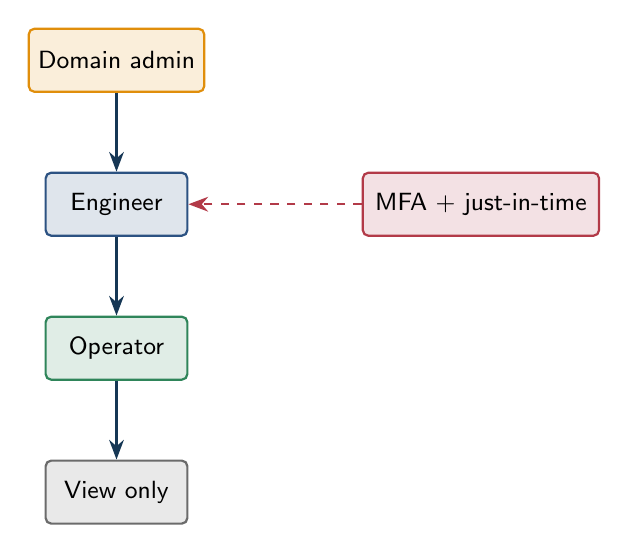
\begin{tikzpicture}[node distance=10mm]
  \node[isbox, fill=isAccent!15, draw=isAccent] (admin) {Domain admin};
  \node[isbox, fill=isPLC!15, draw=isPLC, below=of admin] (eng) {Engineer};
  \node[isbox, fill=isHMI!15, draw=isHMI, below=of eng] (op) {Operator};
  \node[isbox, fill=isMute!15, draw=isMute, below=of op] (view) {View only};
  \node[isbox, fill=isAttack!15, draw=isAttack, right=22mm of eng, minimum width=30mm] (mfa) {MFA + just-in-time};
  \draw[flow] (admin) -- (eng);
  \draw[flow] (eng) -- (op);
  \draw[flow] (op) -- (view);
  \draw[flow, dashed, isAttack] (mfa.west) -- (eng.east);
\end{tikzpicture}
\par\vspace{2mm}
\footnotesize Per-person accounts, no shared logins. Keep a local fallback in case AD goes down.
\note{
  Role separation in OT collapses for one reason: the shared ``operator'' login on the control-room HMI. Operators rotate shifts, gloves are on, and nobody types a password at 3 a.m. -- so an icon on the desktop auto-logs in. That is reality. Push MFA where it works (jump hosts, engineering downloads, AD admin) and accept a kiosk-style HMI session with strong \emph{physical} access control around the room. Just-in-time elevation via something like CyberArk or BeyondTrust beats permanent domain admin every time. Class question: where in this hierarchy would you put a vendor support engineer who shows up twice a year?
}
\end{frame}

\begin{frame}{Secure Remote Access Pattern}
\centering
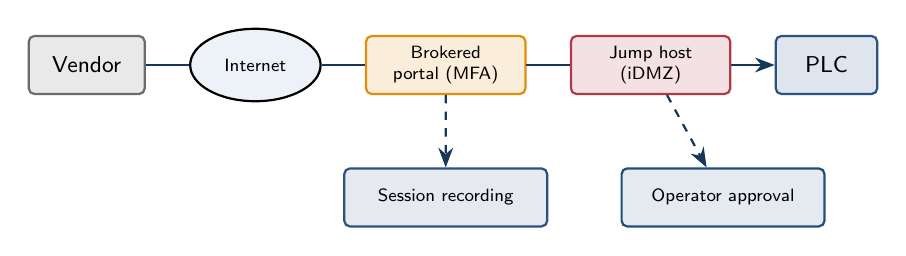
\begin{tikzpicture}[node distance=6mm, scale=0.92, transform shape]
  \node[isbox, fill=isMute!15, draw=isMute, minimum width=16mm] (vend) {Vendor};
  \node[inetnode, fill=isLight, minimum width=18mm, right=of vend] (inet) {Internet};
  \node[isbox, fill=isAccent!15, draw=isAccent, right=of inet, align=center, minimum width=22mm, font=\scriptsize] (broker) {Brokered\\portal (MFA)};
  \node[isbox, fill=isAttack!15, draw=isAttack, right=of broker, align=center, minimum width=22mm, font=\scriptsize] (jump) {Jump host\\(iDMZ)};
  \node[plc, right=of jump, minimum width=14mm] (target) {PLC};
  \node[isbox, fill=isPLC!12, draw=isPLC, below=10mm of broker, font=\scriptsize, minimum width=28mm] (rec) {Session recording};
  \node[isbox, fill=isOT!12, draw=isOT, below=10mm of jump, font=\scriptsize, minimum width=28mm, xshift=10mm] (appr) {Operator approval};
  \draw[flow] (vend) -- (inet) -- (broker) -- (jump) -- (target);
  \draw[flow, dashed] (broker) -- (rec);
  \draw[flow, dashed] (jump) -- (appr);
\end{tikzpicture}
\note{
  This is the pattern that actually scales for vendor support. The broker (Cyolo, BeyondTrust Privileged Remote Access, Claroty SRA) terminates the vendor session in the iDMZ; the jump host is the only thing that talks to the PLC, and every keystroke is recorded. The \emph{operator approval} arrow is the cultural change -- a vendor cannot just connect, an on-shift operator clicks ``allow'' for this 30-minute window. War story: a turbine vendor ran a flat IPsec VPN straight into Level 2 for ten years; the day they were breached, the customer's plant was on the same broadcast domain. Compare this slide with what your plant actually has today.
}
\end{frame}

\section{Patching, Backups, Monitoring}

\begin{frame}{Patching Strategy in OT}
\centering
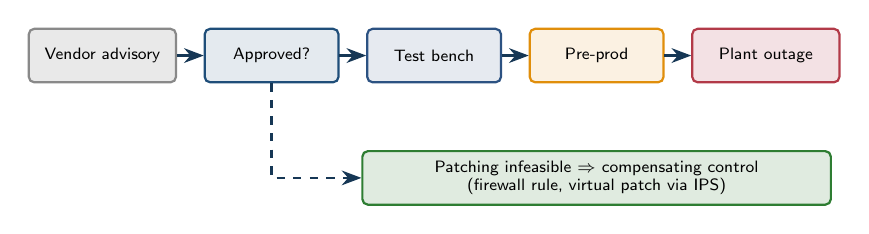
\begin{tikzpicture}[node distance=4mm, scale=0.85, transform shape]
  \node[server, minimum width=22mm, font=\scriptsize] (vend) {Vendor advisory};
  \node[isbox, fill=isOT!12, draw=isOT, right=of vend, minimum width=20mm, font=\scriptsize] (apv) {Approved?};
  \node[isbox, fill=isPLC!12, draw=isPLC, right=of apv, minimum width=20mm, font=\scriptsize] (test) {Test bench};
  \node[isbox, fill=isAccent!12, draw=isAccent, right=of test, minimum width=20mm, font=\scriptsize] (stage) {Pre-prod};
  \node[isbox, fill=isAttack!15, draw=isAttack, right=of stage, minimum width=22mm, font=\scriptsize] (prod) {Plant outage};
  \node[isbox, fill=isNet!15, draw=isNet, below=10mm of stage, minimum width=70mm, font=\scriptsize, align=center] (cc)
    {Patching infeasible $\Rightarrow$ compensating control\\(firewall rule, virtual patch via IPS)};
  \draw[flow] (vend) -- (apv);
  \draw[flow] (apv) -- (test);
  \draw[flow] (test) -- (stage);
  \draw[flow] (stage) -- (prod);
  \draw[flow, dashed] (apv.south) |- (cc.west);
\end{tikzpicture}
\note{
  The IT instinct is ``patch Tuesday.'' OT cannot. Vendor-approved is the gate: Siemens, Rockwell, ABB, Honeywell each publish which Microsoft KBs they have validated against their stack, and applying anything else can void support. The test bench and pre-prod stages are where you catch the patch that breaks the OPC server. The \emph{compensating control} branch is the honest answer for the 60\% of assets you will never patch -- a tighter firewall ACL, a Snort/Suricata signature on the IDS, an IPS rule in front of a vulnerable HMI. Ask the room: how long is acceptable between a CISA advisory and \emph{some} mitigation in your plant?
}
\end{frame}

\begin{frame}{Backups -- 3-2-1 (and Immutable)}
\centering
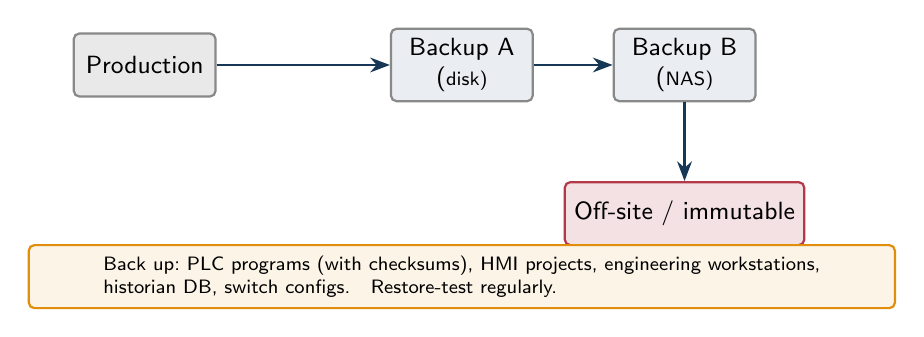
\begin{tikzpicture}[node distance=10mm]
  \node[server] (prod) {Production};
  \node[server, fill=isPLC!10, right=22mm of prod] (b1) {Backup A\\(\scriptsize disk)};
  \node[server, fill=isPLC!10, right=of b1] (b2) {Backup B\\(\scriptsize NAS)};
  \node[server, fill=isAttack!15, draw=isAttack, below=of b2] (b3) {Off-site / immutable};
  \draw[flow] (prod) -- (b1);
  \draw[flow] (b1) -- (b2);
  \draw[flow] (b2) -- (b3);
  \node[isbox, fill=isAccent!10, draw=isAccent, below=18mm of b1, font=\scriptsize, minimum width=110mm, align=left]
    {Back up: PLC programs (with checksums), HMI projects, engineering workstations,\\
     historian DB, switch configs.\quad Restore-test regularly.};
\end{tikzpicture}
\note{
  3-2-1 is the floor. The ransomware era added \emph{immutable} -- either write-once media or S3 Object Lock / Veeam hardened repository, so an attacker with domain admin cannot wipe the backups. Backing up PLC programs sounds obvious but is routinely missed: the only copy of the ladder logic lives on an engineer's laptop, with no checksum and no version control. Same for HMI projects, historian databases, and switch configs (push to RANCID / Oxidized). The restore-test bullet is where most programs fail -- a backup you have never restored is a hope, not a backup. War story: a water utility paid the ransom in 2021 because their tapes had been spinning untested for two years and the catalog was corrupt.
}
\end{frame}

\begin{frame}{Passive OT IDS Placement}
\centering
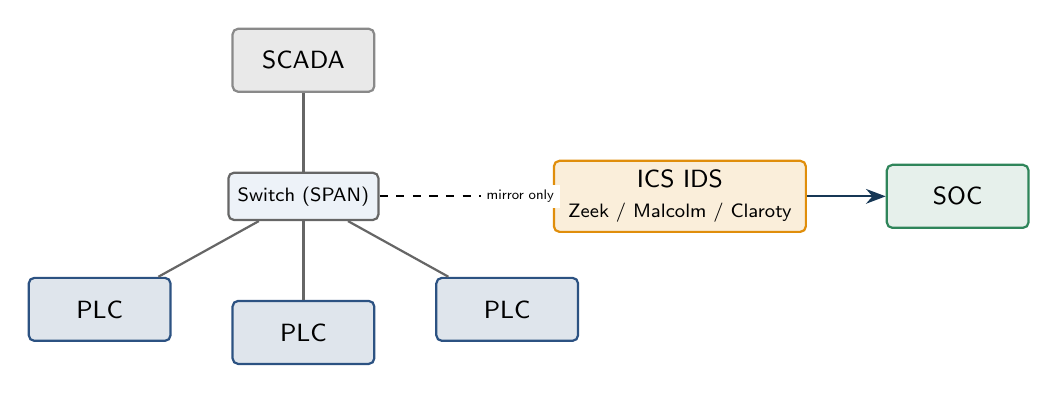
\begin{tikzpicture}[node distance=10mm]
  \node[server] (scada) {SCADA};
  \node[switch, below=of scada] (sw) {Switch (SPAN)};
  \node[plc, below left=of sw] (p1) {PLC};
  \node[plc, below=of sw] (p2) {PLC};
  \node[plc, below right=of sw] (p3) {PLC};
  \node[isbox, fill=isAccent!15, draw=isAccent, right=22mm of sw, minimum width=32mm] (ids) {ICS IDS\\\scriptsize Zeek / Malcolm / Claroty};
  \node[server, right=of ids, fill=isHMI!12, draw=isHMI] (soc) {SOC};
  \draw[netline] (scada) -- (sw);
  \foreach \n in {p1,p2,p3}{\draw[netline] (\n) -- (sw);}
  \draw[-{Stealth[length=2mm]}, dashed, thick] (sw) -- node[midway, right=5pt, font=\tiny, fill=white, inner sep=2pt]{mirror only} (ids);
  \draw[flow] (ids) -- (soc);
\end{tikzpicture}
\source{Tools: Zeek (Paxson, 1999); Malcolm (Idaho National Lab); commercial: Claroty CTD, Nozomi Guardian, Dragos Platform.}
\note{
  Passive means \emph{passive} -- the IDS sits on a SPAN port or a hardware TAP and never injects a packet. That is the only thing the safety case will accept on Purdue Level 2. The placement detail people miss is which VLAN the SPAN actually carries: I have seen a Nozomi Guardian deployed for a year that was mirroring only the management VLAN, not the process VLAN, so it saw zero Modbus. Verify with \texttt{tcpdump -i} before declaring victory. Zeek plus Suricata in Malcolm is a credible open-source stack; Claroty CTD, Nozomi Guardian, Dragos Platform, Cisco Cyber Vision, and Forescout SilentDefense are the commercial options -- the differentiator is the protocol dissector library, not the UI.
}
\end{frame}

\begin{frame}{What an OT IDS Looks For}
\centering
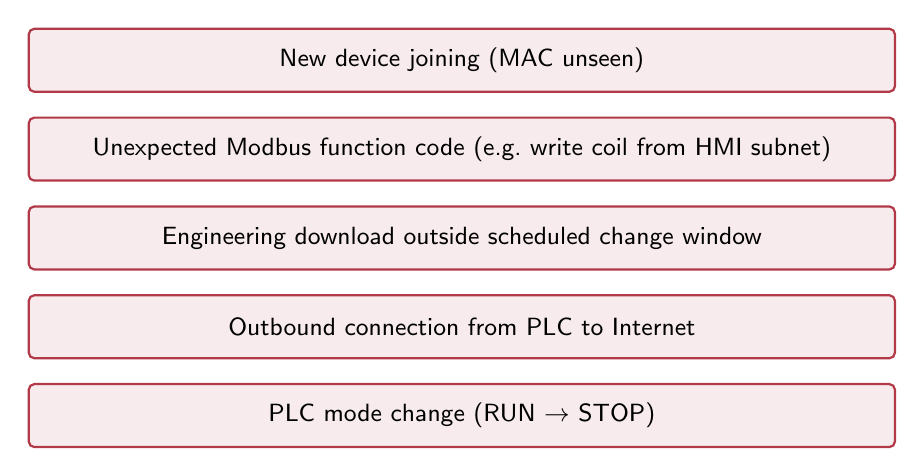
\begin{tikzpicture}[node distance=3mm]
  \node[isbox, fill=isAttack!10, draw=isAttack, minimum width=110mm, font=\small] (a) {New device joining (MAC unseen)};
  \node[isbox, fill=isAttack!10, draw=isAttack, minimum width=110mm, font=\small, below=of a] (b) {Unexpected Modbus function code (e.g.\ write coil from HMI subnet)};
  \node[isbox, fill=isAttack!10, draw=isAttack, minimum width=110mm, font=\small, below=of b] (c) {Engineering download outside scheduled change window};
  \node[isbox, fill=isAttack!10, draw=isAttack, minimum width=110mm, font=\small, below=of c] (d) {Outbound connection from PLC to Internet};
  \node[isbox, fill=isAttack!10, draw=isAttack, minimum width=110mm, font=\small, below=of d] (e) {PLC mode change (RUN $\rightarrow$ STOP)};
\end{tikzpicture}
\note{
  These five signatures are the ``free'' detections you get the day you deploy any OT IDS. Asset discovery alone -- a new MAC on the process VLAN -- catches the contractor laptop and the rogue access point. The unexpected Modbus function code is the Stuxnet-shaped detection: writes from a subnet that has historically only read. Engineering downloads outside a change window directly maps to your management-of-change process and turns a security alert into a safety conversation. The PLC RUN-to-STOP transition is the one your operations team will care about more than you do -- get them subscribed to that alert before you even tune the rest.
}
\end{frame}

\begin{frame}{Network Access Control (NAC) in OT}
\centering
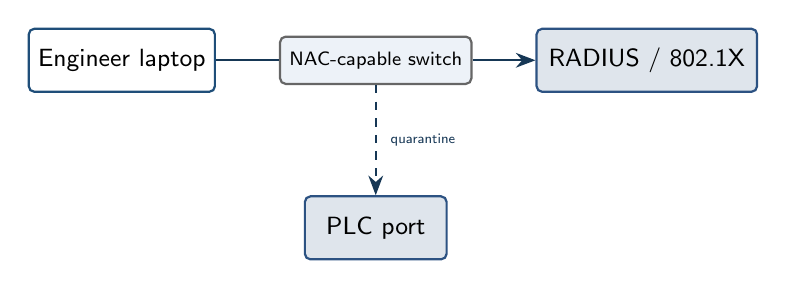
\begin{tikzpicture}[node distance=8mm]
  \node[workstation] (lap) {Engineer laptop};
  \node[switch, right=of lap] (sw) {NAC-capable switch};
  \node[server, fill=isPLC!15, draw=isPLC, right=of sw, minimum width=28mm, font=\small] (auth) {RADIUS / 802.1X};
  \node[plc, below=14mm of sw] (plc) {PLC port};
  \draw[flow] (lap) -- (sw) -- (auth);
  \draw[flow, dashed] (sw) -- node[midway, right=4pt, font=\tiny, fill=white, inner sep=1pt]{quarantine} (plc);
\end{tikzpicture}
\vspace{2mm}
\begin{notebox}{Sealing the wall jack}
802.1X (with MAC bypass for legacy devices) prevents random laptops from joining the plant LAN. Static PLC ports get MAC pinning.
\end{notebox}
\source{IEEE 802.1X-2020 \textbar{} NIST SP 800-92 (logging) \textbar{} vendors: Cisco ISE, Aruba ClearPass, Forescout eyeSight.}
\note{
  802.1X in OT is the long-running argument. The clean version requires a supplicant on every endpoint -- and a Siemens S7-1500 does not speak EAP. The workable version is MAC Authentication Bypass with a Forescout SilentDefense or Cisco ISE policy that pins each PLC port to a known OUI and quarantines anything else. Profile the device before you let it on, not after. The Stuxnet-era lesson is that the attack came in on a USB, but the lateral move was over the flat plant LAN with no port security at all. Ask the room: what is your move when an engineer's laptop fails 802.1X at 2 a.m. during an outage?
}
\end{frame}

\begin{frame}{USB Allow-Listing}
\centering
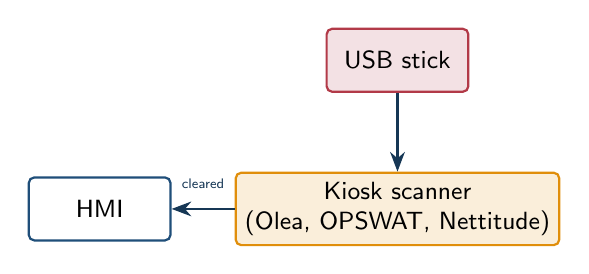
\begin{tikzpicture}[node distance=8mm]
  \node[workstation] (ws) {HMI};
  \node[isbox, fill=isAccent!15, draw=isAccent, right=of ws, minimum width=40mm, font=\small, align=center] (kiosk) {Kiosk scanner\\(Olea, OPSWAT, Nettitude)};
  \node[isbox, fill=isAttack!15, draw=isAttack, font=\small, above=10mm of kiosk] (usb) {USB stick};
  \draw[flow] (usb) -- (kiosk);
  \draw[flow] (kiosk) -- node[midway, above=5pt, font=\tiny, fill=white, inner sep=2pt]{cleared} (ws);
\end{tikzpicture}
\vspace{2mm}
\begin{importantbox}{One door}
Every USB must pass through one of N approved scanning kiosks before it touches an HMI. Block all other USB at the OS level.
\end{importantbox}
\note{
  ``We banned USB'' is the common claim -- until the vendor walks in with a firmware update on a stick and a deadline. The kiosk approach (OPSWAT MetaDefender, Olea Renegade, Nettitude USB sanitiser) is the realistic compromise: scan with 8+ AV engines, strip macros, re-emit onto a sanitised stick. War story: a refinery had a kiosk in the gatehouse that was bypassed for two years because the operators discovered it stopped scanning when a specific drive letter was already mounted; nobody checked the logs. Block USB at the OS layer via Group Policy or McAfee Device Control \emph{as well}, so the kiosk is the only viable path. Otherwise the policy is theatre.
}
\end{frame}

\begin{frame}{Logging Strategy for OT}
\centering
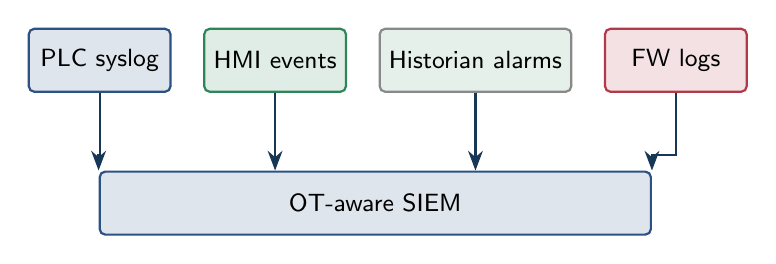
\begin{tikzpicture}[node distance=4mm]
  \node[plc] (a) {PLC syslog};
  \node[hmi, right=of a] (b) {HMI events};
  \node[server, right=of b, fill=isHMI!12] (c) {Historian alarms};
  \node[firewall, right=of c] (d) {FW logs};
  \node[server, fill=isPLC!15, draw=isPLC, below=14mm of {$(b)!0.5!(c)$}, minimum width=70mm, font=\small] (siem) {OT-aware SIEM};
  \draw[flow] (a.south) |- ([yshift=2mm]siem.north west) -- (siem.north west);
  \draw[flow] (b.south) -- (b.south |- siem.north);
  \draw[flow] (c.south) -- (c.south |- siem.north);
  \draw[flow] (d.south) |- ([yshift=2mm]siem.north east) -- (siem.north east);
\end{tikzpicture}
\vspace{2mm}
\begin{notebox}{Send everything, correlate centrally}
Most ICS devices have weak logging -- compensate with network IDS and host-based agents on the windows-class assets.
\end{notebox}
\note{
  The most expensive misconception in this section is ``we have a SIEM.'' Splunk, Elastic, or IBM QRadar do not natively parse IEC 60870-5-104, DNP3, or S7Comm -- without an OT add-on (Splunk OT Add-on, Dragos Platform feed, Claroty XDR integration) you are correlating Windows event IDs and calling it OT visibility. Send PLC syslog where you can, HMI Windows events, historian alarms, firewall logs, and the IDS metadata into one place. Then build a handful of correlation rules that cross IT and OT signals -- e.g.\ a successful jump-host login followed within five minutes by an engineering download. Without correlation a SIEM is a very expensive log archive.
}
\end{frame}

\begin{frame}{Deception in OT}
\begin{itemize}
  \item Honey-PLCs / honey-HMIs lure scans and exploit attempts.
  \item Decoy credentials (canary tokens) trip alerts when used.
  \item Fake assets in DNS / Active Directory.
  \item False engineering-WS hostnames as tripwires.
\end{itemize}
\begin{tipbox}{Low cost, high signal}
A honey-PLC sees \emph{zero} legitimate traffic by design -- any hit is a near-certain incident.
\end{tipbox}
\note{
  Deception is the cheapest detection control you will deploy. Conpot is the open-source honey-PLC, Thinkst Canary sells a turnkey appliance, and a canary token in a fake \texttt{plc\_credentials.txt} on the engineering share costs nothing. The point is the false-positive rate: a honey-PLC at \texttt{10.20.5.99} sees \emph{zero} legitimate traffic by design, so a single TCP/502 probe is a near-certain incident -- no tuning, no triage. Drop a few across each process VLAN, name them in line with your real assets (\texttt{LINE3-PLC-07}), and wire the alert straight to the on-call channel. Bridge: next section we move from defending the plant to detecting and responding when one of these tripwires fires.
}
\end{frame}

\begin{frame}{Summary -- Section \sectionNumber}
\begin{takeawaybox}{What to remember from this section}
\begin{itemize}\setlength{\itemsep}{2pt}
  \item Defense in depth layers people, process, and technology.
  \item Hardening and application whitelisting fit well on static HMIs.
  \item Brokered, recorded, approved remote access beats open VPNs to the plant.
  \item Passive OT IDS provides visibility without injecting traffic into production.
\end{itemize}
\end{takeawaybox}
\note{
  Close on the independence theme. The four takeaways are the minimum bar; the real test is whether your layers fail independently. If your IDS, your SIEM, and your jump host all log into the same Active Directory with the same admin account, the attacker who owns AD owns all three. Push the class on a final question: pick \emph{one} layer from today's deck that you would add to a brownfield plant first, and justify it on cost-per-detection. Next section we leave prevention behind and look at detection, response, and recovery -- because everything in this deck eventually fails, and the question is how fast you notice.
}
\end{frame}

\referencesframe{
  \item Idaho National Lab. \emph{Recommended Practice: Improving Industrial Control System Cybersecurity with Defense-in-Depth Strategies}, 2016.
  \item NIST SP 800-82 Rev.\,3. \emph{Guide to OT Security}, Sep 2023.
  \item CIS. \emph{CIS Critical Security Controls} v8, 2021.
  \item CIS Benchmarks (Windows, Linux). Center for Internet Security.
  \item NIST SP 800-167. \emph{Guide to Application Whitelisting}, 2015.
  \item NIST SP 800-92. \emph{Guide to Computer Security Log Management}, 2006.
  \item IEEE 802.1X-2020. \emph{Port-based network access control}.
  \item Paxson, V. ``Bro: A System for Detecting Network Intruders in Real-Time.'' \emph{Computer Networks}, 1999 (Zeek origin).
  \item Open Information Security Foundation. \emph{Suricata IDS}, \url{https://suricata.io}.
  \item Idaho National Lab. \emph{Malcolm} network monitor, \url{https://github.com/idaholab/Malcolm}.
  \item NIST SP 800-46. \emph{Guide to Enterprise Telework, Remote Access, and BYOD Security}, 2016.
  \item CISA. \emph{Recommended Cybersecurity Practices for Industrial Control Systems}, 2020.
}

\closingframe

\end{document}
